\chapter{MVC in IBM Content Navigator}
\label{chap:nexus}
This chapter introduces the IBM Content Navigator application and framework. After an overview on its architecture and plug--in system, the main client-side components Dojo and \ac{idx} are outlined. To conclude this chapter, the design and implementation of a log analysis plug--in is discussed.
\section{Architecture and Extension Points}
IBM Content Navigator is an enterprise web application written in Java and JavaScript. The server--side part is designed to run on a \ac{j2ee} application server, the client--side part runs in a web browser. The architecture of Content Navigator, which is presented here, allows the extension through plug--ins at many points of the application.

\subsection{Architecture: Layers and Components}
IBM Content Navigator is designed after the \emph{Separation of Concerns} principle. This is true for the different layers of Content Navigator on the one hand, and the different tiers it uses on the other hand. The layers of ICN are shown in Figure~\ref{fig:nexuslayers}.

\begin{figure}[H]
	\centering
	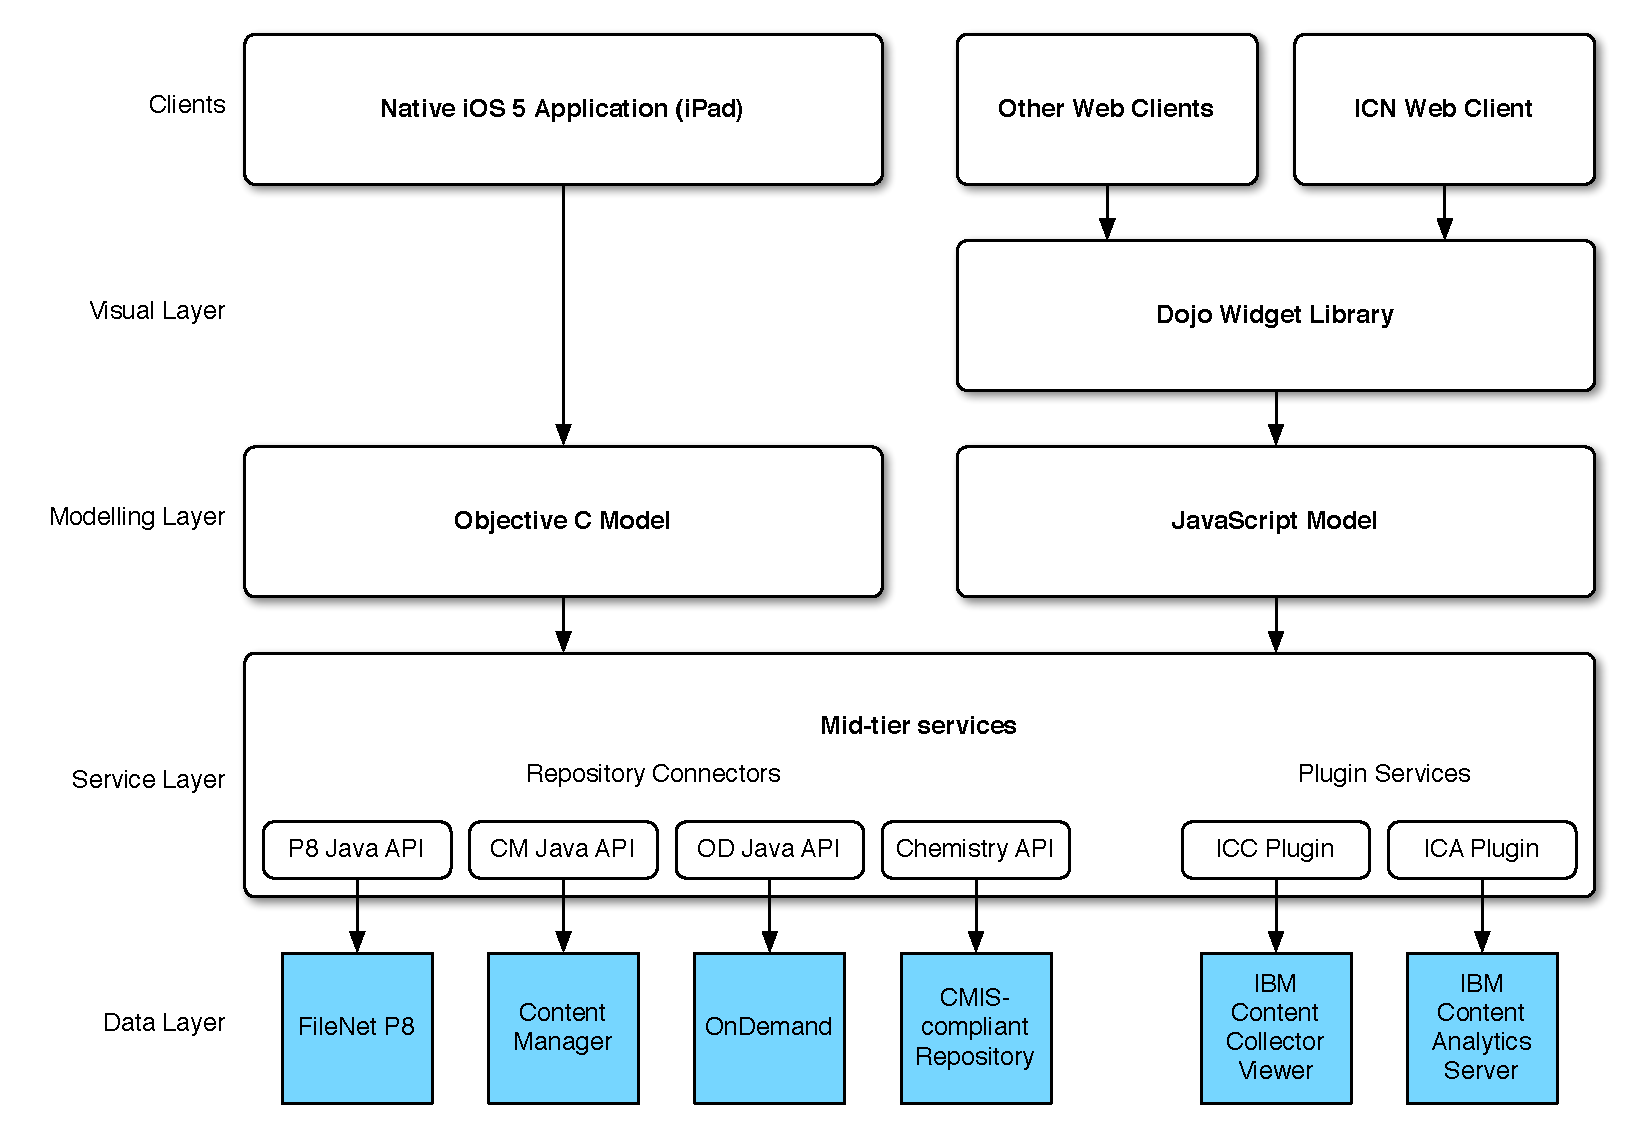
\includegraphics[width=16cm]{images/layers.pdf}
	\caption{Layers of IBM Content Navigator}
	%\captionsetup{font={footnotesize,bf,it}}
	%\caption*{Source: \cite[p. 5]{gof}}
	\label{fig:nexuslayers}
\end{figure}

The top layer represents the actual clients for Content Navigator. Besides the desktop web client, there exists also a mobile iOS 5 client, which is not in the scope of this thesis. The client layer makes use of the visual layer underneath that contains all the Dojo widgets (\emph{Dijits}). In turn, the widgets access the modelling layer, which contains JavaScript Models held in the browser. On the one hand, these models can be connected to mid-tier services, such as ECM repository \glspl{api}, on the other hand, they can be directly connected to external, HTTP-based services, such as \ac{rest}.

The mid-tier services are implemented in Java and run on the application server, whereas the modelling and widget layers run in the browser. This is illustrated by Figure~\ref{fig:nexustiers}, which shows the tier architecture of Content Navigator.

\begin{figure}[H]
	\centering
	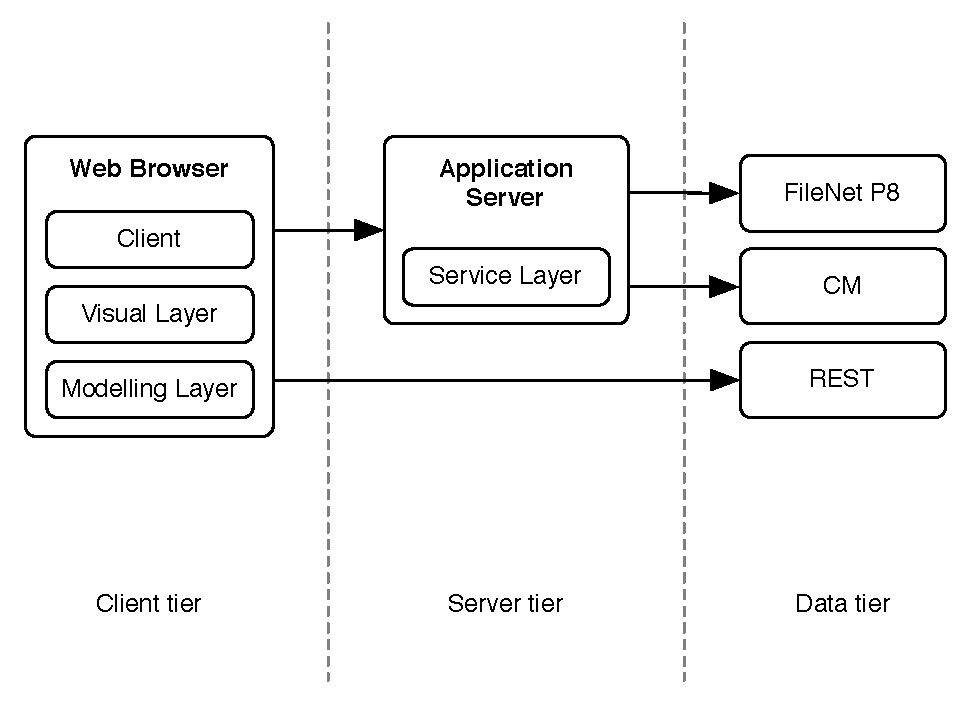
\includegraphics[width=14cm]{images/tiers.pdf}
	\caption{3-Tier architecture of IBM Content Navigator}
	%\captionsetup{font={footnotesize,bf,it}}
	%\caption*{Source: \cite[p. 5]{gof}}
	\label{fig:nexustiers}
\end{figure}

\subsection{Extension Points: Plug--ins}
\label{sec:plugincomponents}
The modular architecture previously presented makes it easy to extend Content Navigator on different levels. Plug--ins for \ac{icn} can include different components that can directly be used inside of \ac{icn}, as described by \citeasnoun**[pp. 103ff.]{redbook}. The ones relevant for the log analysis plug--in are \emph{Plugins} themselves, \emph{Features} and \emph{Widgets}.

\begin{description}
	\item[Plugins] are the containers for the following extension points, which are registered with ICN through the ``Plugin'' Java class.
	\item[Actions] are buttons or menu items that can be triggered by the user; they can be added to the existing \ac{ui} of ICN.
	\item[Menus] of the existing UI can also be created and customized, just like \emph{Actions}.
	\item[Plug--in Services] allow developers to extend the service layer of Content Navigator. They can implement arbitrary Java code, but can be called from the client-side JavaScript as they are exposed by a Servlet.

	Using a \emph{Service}, it is possible to build anything that Java is capable of. This can be, just to name a few examples, a proxy for REST calls, an additional connector to a content repository not already covered by ICN, or a system to save data on the server side. The \ac{ica} plug--in uses \emph{Services} to connect to an ICA server via \ac{sso}.
	\item[Features] are areas of the application \ac{ui}. In ICN, the Browser, Favorites, Team Spaces, Search, Work and Administration \emph{Features} do already exist and can be accessed using the Feature Pane on the left side of the \ac{ui} (when logged in).

	\emph{Features} are associated with a Dojo class to specify the View that should be shown when the \emph{Feature} is accessed.
	\item[Viewers] are used to display the content of a specific document type.
	\item[Layouts] can customize the overall layout of the application \ac{ui}, whereas \emph{Features} can only define a certain application area. ICN's standard layout (Banner Bar at the top, Global Menu below, Feature Pane on the left and Features filling the remaining screen space) can be changed using \emph{Layouts}.
	\item[Request and Response Filters] are used to change the JSON sent from and received by \emph{Services}.
	\item[Widgets] are Dojo Dijits that can be included in Plug-ins. They can either be developed from scratch or extend already existing Dojo or IDX Dijits. More on Dijits is written in Section~\ref{sec:dojo}.
\end{description}

Besides these components, arbitrary JavaScript code, best created as Dojo modules, can be written and packaged into the plug--in. This includes Model and Controller code. Figure~\ref{fig:plugincomponents} illustrates the connection between extension points and the ICN layer architecture (please compare to Figure~\ref{fig:nexuslayers}).

\begin{figure}[H]
	\centering
	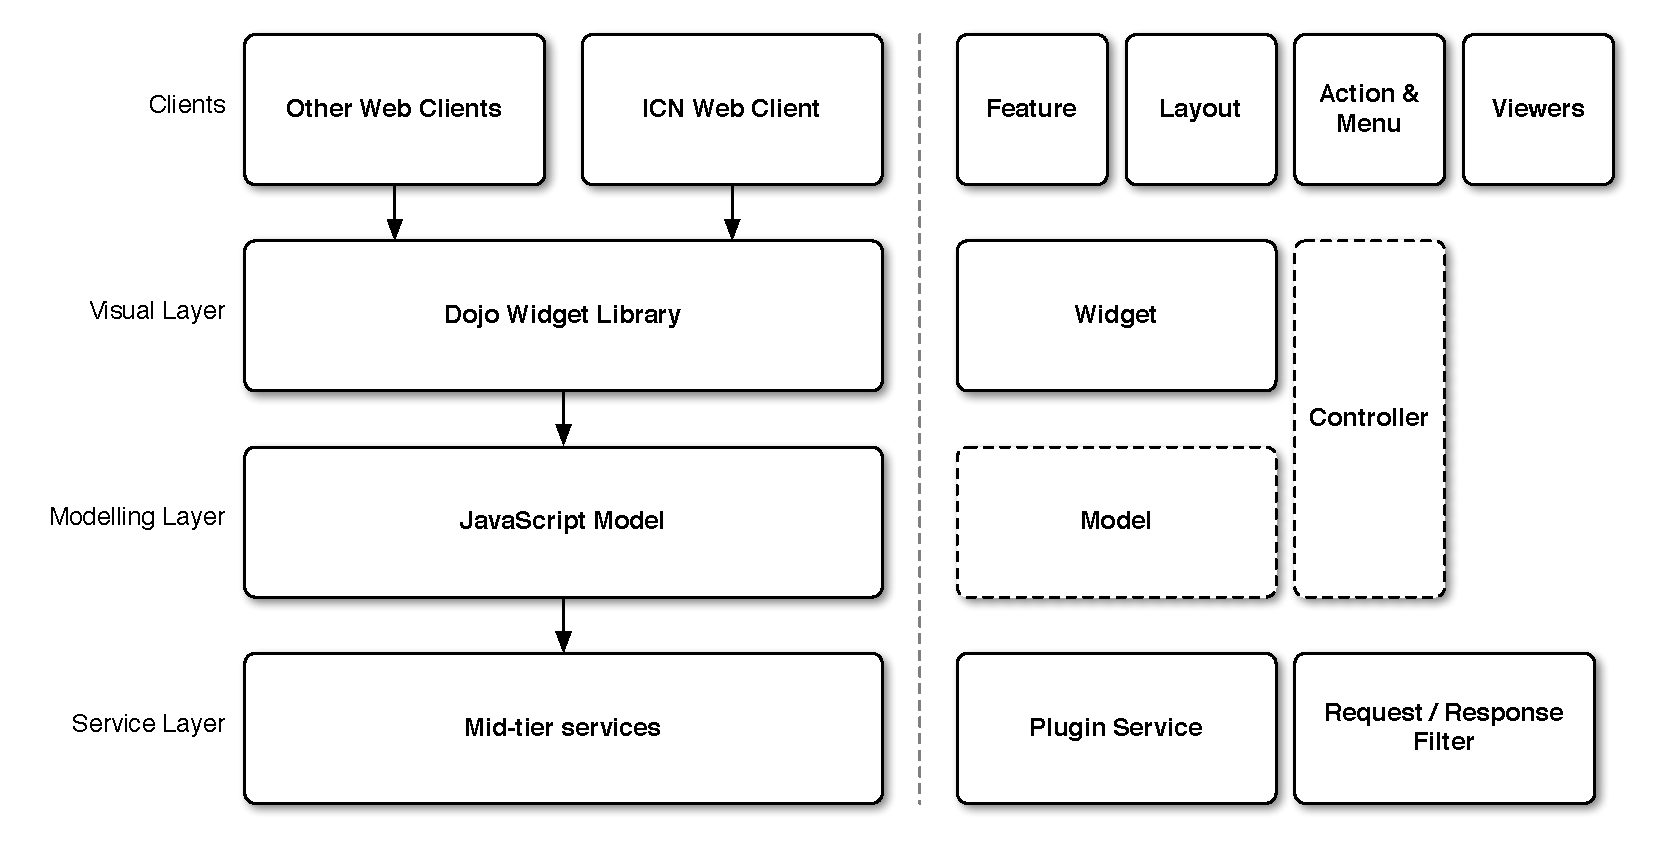
\includegraphics[width=16cm]{images/plugincomponents.pdf}
	\caption{Plug--in components extending ICN}
	\label{fig:plugincomponents}
\end{figure}

As can be seen, plug--ins cannot extend the data layer, as it is not part of \acl{icn} itself, but rather composed of external data sources, such as content repositories and REST services.

\subsection{Deployment and Configuration}
Content Navigator itself is packaged --- without any plug--ins --- into an \ac{ear} file and can directly be deployed on an application server, such as IBM \acl{was}. The connection to a \gls{db2} database for storing and loading the configuration is needed and can be set up using the ICN initialization tool.

Plug--ins are deployed separately. They are packaged as \ac{jar} files and placed at any location that is accessable via a \ac{url}. Plug--ins can be loaded using the administration pane of \ac{cn}. This separation between the actual application and its plug--ins allows the application administrator to update, load and unload plug--ins without restarting \ac{cn} or the application server.

Different ICN-based applications, called \emph{Desktops}, can run on the same ICN installation. A Desktop can be configured using the ICN administration pane; it is assigned a \emph{Layout} and a number of \emph{Features} (as described in Section~\ref{sec:plugincomponents}), as well as content repositories and other options. A Desktop is chosen via the URL, for example \code{http://localhost/navigator?desktop=sccm}. Figure~\ref{fig:nexusapps} illustrates how applications can be assembled using \emph{Features} of different plug--ins.

\begin{figure}[H]
	\centering
	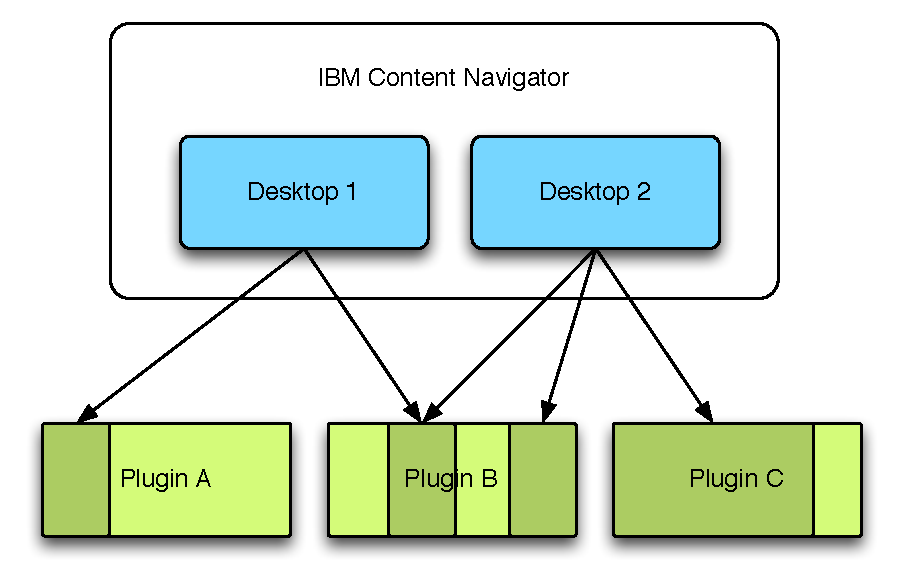
\includegraphics[width=10cm]{images/nexusapps.pdf}
	\caption{ICN Applications using different Plug--in Features}
	\label{fig:nexusapps}
\end{figure}

\section{Dojo Model--View--Controller}
\label{sec:dojo}
This section introduces the components of Dojo that are relevant to building \acl{mvc} applications, and those that were especially used while building the log analysis plug--in for \ac{sccm}. As IBM Content Navigator 2.0 (which is the latest version as of September 2012) includes Dojo 1.6, this is the version of Dojo referred to in this section.

\subsection{Dojo Basics}
The Dojo Toolkit, usually just called \emph{Dojo}, is a set of libraries to build JavaScript applications. In opposite to other JavaScript libraries, such as jQuery, Prototype or Mootools, Dojo is not only aimed at simplifying \ac{dom} manipulation, \ac{ajax} and event handling, but also comes with an extensive widget library (\emph{Dijit}) and graphics/charts \ac{api}.

Dojo is separated into three packages:
\begin{description}
	\item[Dojo] is the core package and contains basic functionality, such as \ac{dom} manipulation, \ac{ajax}, effects, and JavaScript language helpers. Its \gls{namespace} is \code{dojo}.
	\item[Dijit] contains all stable widgets, such as layout widgets, forms, dialogs, and a tree view. Its namespace is \code{dijit}.
	\item[DojoX] are the Dojo extensions in the namespace \code{dojox}. This package contains less common components, such as the graphing and charting \ac{api}. The DataGrid (\code{dojox.grid.DataGrid}) and JsonRestStore (\code{dojox.data.JsonRestStore}), which are part of DojoX, are further discussed in Section~\ref{sec:loganal}.
\end{description}

% TODO: eventuell Dojo module beschreiben?

\subsubsection{Classes and Objects}
JavaScript is a prototype-based object-oriented programming language. Dojo simulates class-based object orientation, which is more familiar to developers used to Java, C++, C\# and other languages. To illustrate this, Listing~\ref{lst:classes} contains the declaration of a Dojo class using \code{dojo.declare}.

\begin{listing}[H]
\begin{minted}[linenos=true,frame=none]{javascript}
dojo.declare("my.Thinger", null, {
  constructor: function(/* Object */args){
    dojo.safeMixin(this, args);
  }
});
\end{minted}
\caption{Declaring a Dojo class}
\label{lst:classes}
\end{listing}

This listing declares the \code{my.Thinger} class (in the \code{my} namespace). When instantiating an object, the constructor mixes the \code{args} argument, which should be a JavaScript object, into the new instance. The result of this mixin is shown in Listing~\ref{lst:mixin}.

\begin{listing}[H]
\begin{minted}[linenos=true,frame=none]{javascript}
var thing = new my.Thinger({ count:100 });
console.log(thing.count);
\end{minted}
\caption{Instantiating an object using a Dojo class}
\label{lst:mixin}
\end{listing}

The object\footnote{JavaScript objects can simply be created as literals. Object literals are enclosed in braces (`\{' and `\}') and contain a comma-separated list of properties (attributes and methods).} provided as an argument to the \code{my.Thinger()} constructor is mixed into the new object \code{thing}. This means, that \code{thing} now contains the properties of this object, which can be proven by printing out \code{thing.count} in the console.

All Dojo components, including Dijits, are created using this concept, and so are the classes developed for the log analysis plug--in.

\subsubsection{Scope}
Another of Dojo's concepts being of help in \ac{mvc} applications and the plug--in is \code{dojo.hitch}. The JavaScript \ac{api} of web browsers features a callback-based event system. This means that callbacks are registered to an event and triggered when the event occurs. A frequently faced problem is that the \gls{callback} function has a different scope than the developer would expect \cite[pp. 53--56 and pp. 180--185]{flanagan}. In JavaScript, this is typically solved using a \emph{closure}, a concept to pass on a given scope to another function. In applications with a lot of callbacks, which may also be depending on each other to execute, closures can have a negative impact on the code maintainability and comprehensibility. \code{dojo.hitch} returns a function that, when executed, has a specified scope, as shown in Listing~\ref{lst:hitch}.

\begin{listing}[H]
\begin{minted}[linenos=true,frame=none]{javascript}
function myCallback() {
  console.log(this.localVariable)
}

dojo.declare("my.Thinger", null, {

  localVariable: "I am in the Thinger scope",
  button: null,

  constructor: function() {
    this.button = new dijit.form.Button({
      label: "Hello"
    });
    dojo.connect(this.button, 'onClick', dojo.hitch(this, myCallback));
  }
});

var thing = new my.Thinger();
\end{minted}
\caption{Instantiating an object using a Dojo class}
\label{lst:hitch}
\end{listing}

This listing first defines a function that acts as a callback and refers a variable (``localVariable'') of its own scope (``this''). The Dojo class declared below introduces said variable and constructs a button. In line 14, the ``onClick'' event is registered with the callback through \code{dojo.hitch(this, myCallback)}. It means that the scope of \code{myCallback} at execution time of the callback is set to what \code{this} has been in line 14.
\subsection{MVC Components}
Dojo provides different components that make it possible to build applications using a MVC architecture. In opposition to JavaScript frameworks that were built towards \emph{structuring} an application using MVC (or a comparable pattern), such as Backbone.js, Ember.js and JavaScriptMVC, Dojo lets the software engineer decide on the architecture.

\subsubsection*{Model}
The modules \code{dojo.data} and \code{dojox.data} provide the data modelling layer. They contain a number of Model equivalents, called \emph{Stores}, all of which implement one or more interfaces to handle data \cite{zyp}:
\begin{itemize}
	\item The \emph{Read API} forces the Store to provide methods and maintain internal structures to expose a Store's data
	\item The \emph{Write API} enables a Store to accept data manipulations
	\item The \emph{Identity API} forces the Store to manage an identifier for each single data item. It must be possible to look up a data item using this unique identifier.
	\item If implementing the \emph{Notification API}, other objects can connect to events that fire when data in the Store are changed (an implementation of the \emph{Observer} pattern).
\end{itemize}

Dojo already implements various stores that serve different purposes and can use a specific data source. The \code{ItemFileReadStore}, for example, takes a file of \ac{json} data as the data source (specified by a \ac{url}). It implements the \emph{Identity} and \emph{Read} APIs, so data can be read, but not written. As the source is a file and data cannot be manipulated, it is not necessary for this store to implement the \emph{Notification} API.

The \code{JsonRestStore} serves a more complex purpose. It is connected to a \ac{rest} service and thus needs to implement both the \emph{Read} and \emph{Write} APIs. But the other two APIs are implemented also --- this is especially important as this store is often used in cooperation with a Dijit, such as the Tree or DataGrid. To keep the Dijits up to date, a notification mechanism as provided by the \emph{Notification API} is necessary (see next section for more information on the Tree and DataGrid).


\subsubsection*{View}
In Dojo, the View usually is a single Dijit or a collection of interrelated Dijits. This section presents two data-centric Dijits that are part of Dojo 1.6.

The \emph{Tree} (\code{dijit.Tree}) is a Dijit to display hierarchical data. It cannot connect directly to a Dojo store, but needs an additional API to handle the nested data model. These API can either be implemented manually by mixing in the according functions into the store when instantiating it, or the store can be wrapped by either one of the already existing \code{TreeStoreModel} and \code{ForestStoreModel}. The first expects a single root item, whereas the second expects multiple root items (thus the name \emph{Forest}).

\begin{figure}[H]
	\centering
	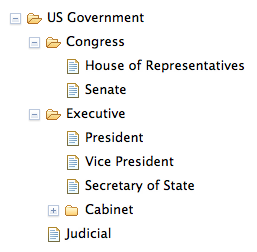
\includegraphics[width=6cm]{images/tree.png}
	\caption{Screenshot of a Dojo Tree}
	%\captionsetup{font={footnotesize,bf,it}}
	%\caption*{Source: \url{http://dojotoolkit.org/documentation/tutorials/1.6/store_driven_tree/}}
	\label{fig:tree}
\end{figure}

Listing~\ref{lst:tree} shows the creation of a store, a TreeStoreModel wrapper around that store and a Tree connecting to the store via the TreeStoreModel. A REST service at the URL \code{data/} is presumed, and the data returned must have a special structure: the attribute ``name'' has to be present in every item, as it is used as the label, and an array with child items has to be placed unter the ``children'' attribute.

Listing~\ref{lst:treejson} shows a sample JSON structure that is returned by the REST service at \code{data/}.

\begin{listing}[H]
\begin{minted}[linenos=true,frame=none]{javascript}
dojo.require("dijit.Tree");
dojo.require("dojox.data.JsonRestStore");
dojo.require("dijit.tree.TreeStoreModel");

store = new dojox.data.JsonRestStore({
  target: "data/"             // URL to the REST service
});

treeModel = new dijit.tree.TreeStoreModel({
  store: store,               // the store to wrap around
  query: {tree:"root"},       // root item
  labelAttr: "name",          // name of the label attribute
  childrenAttrs: ["children"] // attributes holding children
});

tree = new dijit.Tree({       // create a tree
  model: treeModel            // give it our model
}, "tree");                   // target HTML element's id

tree.startup();
\end{minted}
\caption{Creating a Tree with a store and TreeStoreModel}
\label{lst:tree}
\end{listing}



\begin{listing}[H]
\begin{minted}[linenos=true,frame=none]{javascript}
{
  name: "World",
  children: [
    { name: "Africa" },
    { name: "Australia" },
    { name: "Asia" },
    { name: "Europe" },
    { name: "North America",
      children: [
        { name: "Canada" },
        { name: "USA" }
      ]
    },
    { name: "South America" }
  ]
}
\end{minted}
\caption{Sample JSON data for the Tree Dijit}
\label{lst:treejson}
\end{listing}

The \emph{DataGrid} (\code{dojox.grid.DataGrid}) is a Dijit to display tabular data, similar to a spreadsheet. It can be used to display high amounts of data, using features like editable cells, custom cells that contain Dijits or arbitrary HTML code, and lazy loading. Its extension \code{dojox.grid.TreeGrid} can even display hierarchical tabular data using expanders and aggregates.

In opposition to the Tree, the DataGrid can directly access the data of a store. That store has to implement at least the \emph{Read} and \emph{Identity} APIs. The DataGrid also needs a \emph{structure}, which is an object describing the cells of the grid and the source of the cells' data. In the simplest case, a cell can contain the value of an attribute of the according item, but the cell content can also be custom, for example a Dijit or an image.

As the DataGrid is one of the most frequently used Dijits in the log analysis plug--in that was developed in the course of this thesis, an extensive example of implementing it is given later in Section~\ref{sec:plugindesign}.

In Dojo, a View can also be completely built by hand. An example for that is shown in Section~\ref{sec:customview}: a simple, data-displaying IDX Dijit is taken and methods are added to connect it to a Dojo store.

\subsubsection*{Controller}
For the Controller, Dojo does not provide any special classes or APIs. The Controller code can be any code that binds callbacks to View events and performs updates on one or more Models.

An example of a Controller is given in Section~\ref{sec:customview}, which shows the implementation of a custom Model--View--Controller triad using Dojo and the IDX Dijit \code{idx.grid.PropertyGrid}.
%=============================================================================
%=============================================================================
\newpage
\section{Implementation of a Log Analysis Plug--in}
\label{sec:loganal}
In the context of this Bachelor's thesis, a log analysis system was developed by two students. The author created a front-end using \acl{icn}, whereas \citeasnoun{metzger} implemented the respective back-end using \ac{ibm} BigInsights.

\begin{figure}[H]
	\centering
	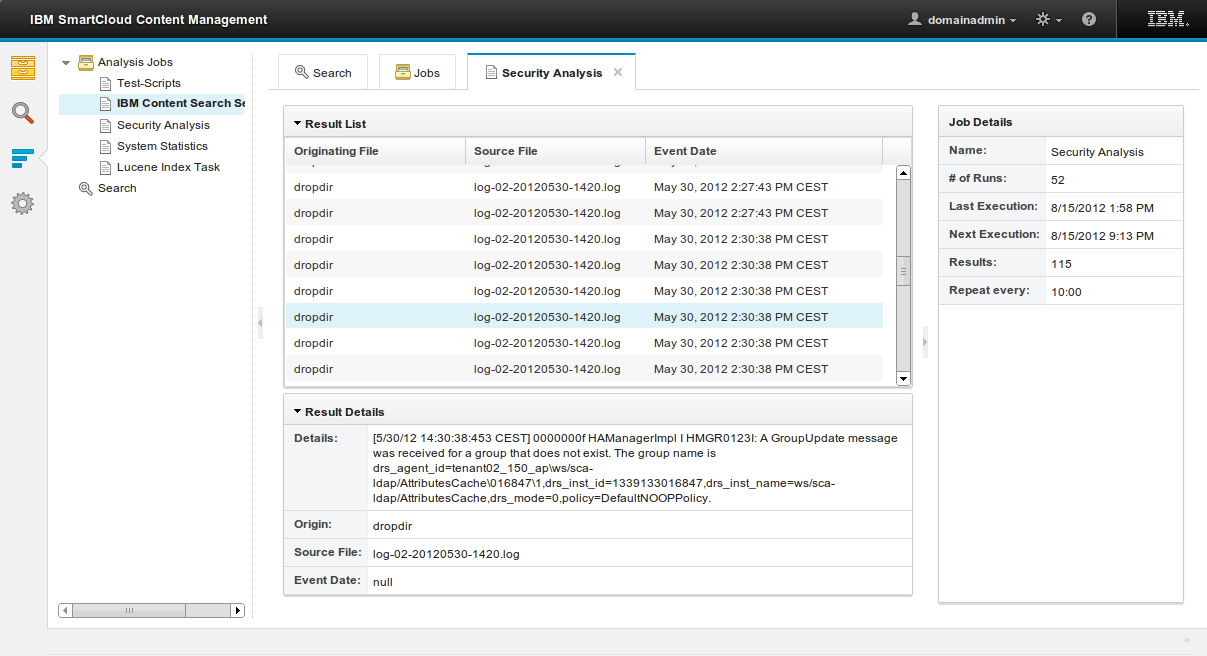
\includegraphics[width=16cm]{screens/job2.png}
	\caption{Screenshot of the log analysis plug--in UI}
	\label{fig:screenshot1}
\end{figure}

\subsection{Motivation}
As part of IBM's \ac{ecm} portfolio, \acl{sccm} is a \acl{saas} for document and email compliance archiving. It is a large integration project that makes use of many IBM software products, such as DB2\footnote{IBM DB2 is a relational database management system (DBMS).}, FileNet P8, \acl{was} and eDiscovery Manager\footnote{IBM \ac{edm} is an ECM product that finds documents related to a specific business case, for example a legal case, in a content repository.}, to provide an out--of--the--box archiving solution to customers. In this cloud environment, massive amounts of operational data are generated in the form of log files, especially if multiple customers are involved.

As \ac{ibm} is responsible for the operation of \ac{sccm}, problems have to be solved immediately as they arise, and steps must be taken to prevent problems beforehand. The large amounts of log data that the integrated software products generate contain knowledge that is necessary for \emph{predictive analysis}. Using IBM BigInsights, correlated log entries can be found and integrated to gain insights on the system's state and arising problems.

These analysis results have to be made available to the cloud operator in an easily accessable manner. Using Content Navigator to develop a front-end for the log analysis system not only makes it possible to integrate it with any ICN based product, but also emphasizes its ability to serve as a flexible, versatile web application framework.

The design and implementation of the BigInsights back-end are not in the scope of this thesis, as they mostly reflect the work of \citeasnoun{metzger}. Nevertheless the interface to the back-end --- a \ac{rest} service --- is presented, as it is essential to some functionality of the front-end.

\subsection{The REST service}
To create a log analysis plug--in and the according REST service, a basic understanding of the data being collected and shown must be present.

Robert Metzger built a data aggregating system using IBM \gls{biginsights}, which is a suite of different products related to \gls{bigdata} analysis. Metzger used different tools out of this suite to create two services: a full-text search for log files and a framework for data aggregation \emph{jobs}. These jobs can be defined using a powerful script language. They run periodically to collect log files, aggregate related log file entries and extract single information out of each collected entry.

Both these services are accessible via a REST service written in Java. The results of both are generated by the BigInsights system and are not meant to be manipulated or deleted by a user. For this reason, the REST service is read--only by design. Strictly spoken, this implementation of REST is incomplete, as there is no \emph{POST}, \emph{PUT} and \emph{DELETE} capability provided.

\subsubsection{Data format}
As the data format for the REST service, JSON was chosen. On the one hand, JSON is flexible without having a lot of overhead (compared to XML), on the other hand, it is natively supported by both the BigInsights products used and JavaScript (and Dojo, respectively). This makes it the preferable data format for this application scenario.

\subsubsection{Services}
The full-text search is available at the REST server's address at the URL \code{/search}. To initiate a query, the GET parameter ``query'' has to be provided with the according query string. A complete query for the string ``security'' looks like this: \code{127.0.0.1/search?query=security}, assuming the REST service runs on localhost\footnote{In IP networks, the IP \code{127.0.0.1} always refers to the \code{localhost}, the very one host that sends the request.}.

As a result, the search service sends a JSON array containing the found log entries as objects. Every object contains the source (the machine and service that wrote the log file), the entry's \gls{timestamp} and the exact log entry content.

The analysis jobs are accessed differently. The URL \code{/jobs} returns a list of all jobs that are known to the system. Besides other attributes, every job has a unique identifier which can be used to further access the job results via \code{/jobs/\%identifier\%}, where \code{\%identifier\%} has to be replaced with the according job identifier.

The list of jobs includes a description of every job. This description consists of metadata, such as the total number of collected results, as well as the structure of a result item. As every job can return completely different data, the client has to know the data structure, the type of every field (e.g. ``date'' or ``integer''), and if the field should be displayed or not. An example of a job description is given in the Appendix on page~\pageref{app:json}.

\subsubsection{Advanced features}
The REST service implements sorting and lazy loading. Both features are built to complement the client-side REST implementation of the \code{dojox.data.JsonRestStore}.

Lazy loading is a form of pagination. But instead of returning a certain ``page'' of data, the REST service returns a ``range''. This range is specified by GET parameters. The store on the client side keeps track of which items are already loaded. It then can request only those that are not loaded, but are needed to be displayed next.

Sorting is also implemented in the REST service on the server side. This may seem inconsequent in a Rich Client application, but it is necessary. Sorting can only be performed if all the data to be sorted are available. As the jobs can return more than 10.000 results, and not all results are loaded on the client due to lazy loading, it is unlikely that the client-side Model contains \emph{all} the items. Because the client would not be able to sort result items correctly if some are missing, sorting is implemented on the server instead.

\subsection{Implementation}
\label{sec:plugindesign}
This section gives a high-level overview on the architecture of the plug--in, especially on the MVC components. Exemplarily, one set of MVC components is presented in more detail.

The log analysis plug--in integrates into IBM Content Navigator and connects to the previously described REST service. The high-level architecture is shown in Figure~\ref{fig:loganalarch}.

\begin{figure}[H]
	\centering
	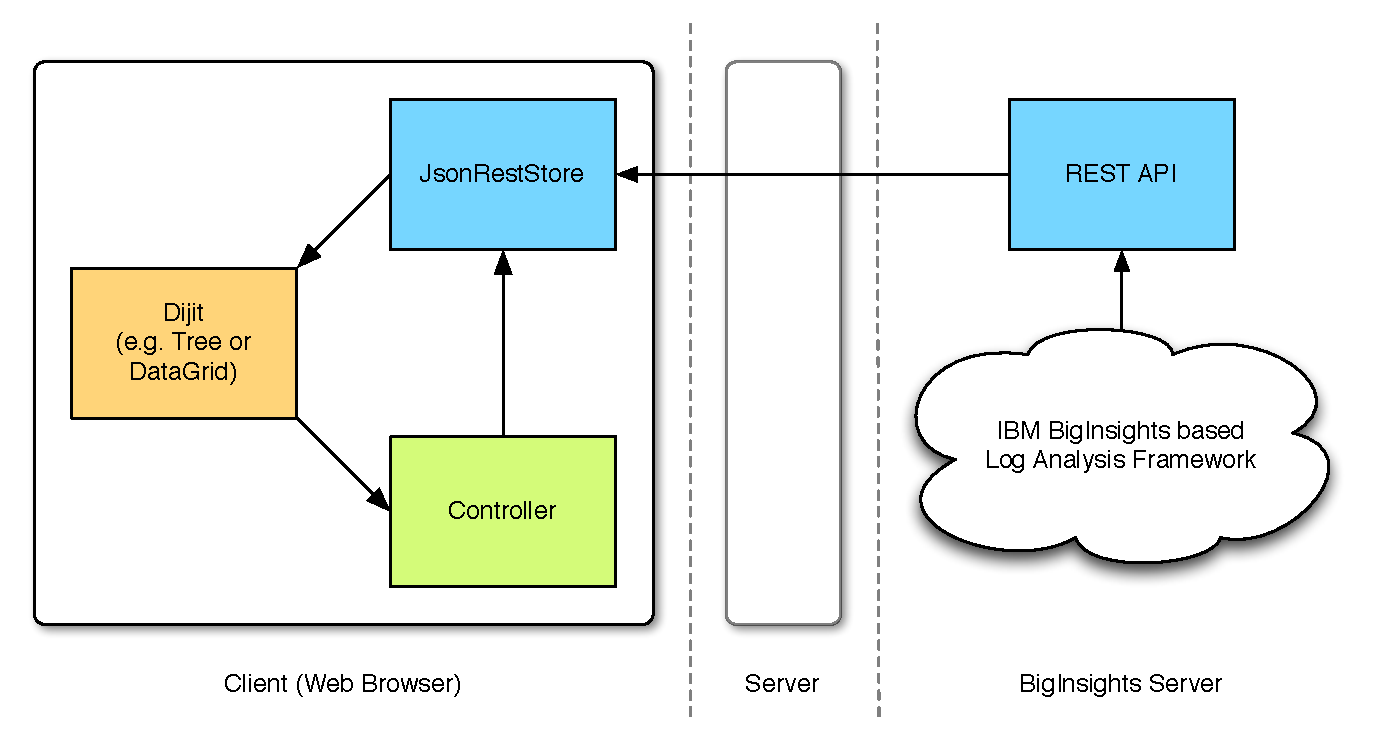
\includegraphics[width=14cm]{images/loganalarch.pdf}
	\caption{Integration of the log analysis plug--in into Content Navigator}
	\label{fig:loganalarch}
\end{figure}

\subsubsection*{File Structure}
The plug--in's \ac{jar} file contains a folder hierarchy, which on the top levels represents the Java package of the plug--ins. The path \pathname{/com/ibm/ecm/extension/sccm/} maps to the Java package \code{com.ibm.ecm.extension.sccm}. It contains two classes, the \code{SCCMPlugin} class, which represents the plug--in object within ICN and contains information on the plug--in components, and the \code{LogAnalysisFeature} class, which represents the \emph{Feature} that is exposed through the plug--in.

One level deeper, the \code{WebContent} folder contains the main \ac{css} and JavaScript files of the plug--in. \code{sccmPlugin.css} contains custom styles needed in the plug--in, while \code{sccmPlugin.js} loads the required Dojo classes using \code{dojo.require()} statements.

The folder hierarchy below \code{WebContent} can partially be mapped to JavaScript namespaces, but also contains additional resources:
\begin{description}
	\item[\code{sccm/layout}] contains Dijits used for layouting in the \code{sccm.layout} namespace
	\item[\code{sccm/model}] contains Models in the \code{sccm.model} namespace
	\item[\code{sccm/view}] contains Dijits used as Views in the \code{sccm.view} namespace
	\item[\code{sccm/resources}] contains images and \ac{css} files
\end{description}
The Dijits developed for the log analysis plug--in are based on \emph{\glspl{template}}, so every folder that contains Dijits also contains a \code{templates} folder with the according HTML files.

\code{sccm/ConfigurationPane.js} is a layout Dijit that gets included in the administration panel of ICN. It can be used to provide configuration options for the plug--in, such as the host and port of the log analysis REST service.

\begin{figure}
	\centering
	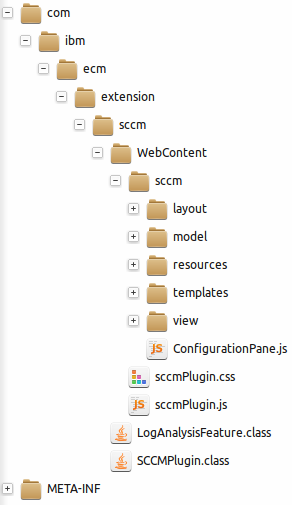
\includegraphics[width=6cm]{screens/folders.png}
	\caption{Folder hierarchy of the log analysis plug--in}
	\label{fig:folders}
\end{figure}

\subsubsection*{User Interface Integration and Layout}
To access the functionality of the log analysis plug--in, a new \emph{Feature} was created. When integrated into a Desktop, this Feature can be accessed using the Feature pane on the left side of the ICN interface.

The layout of the log analysis Feature was created using \emph{container Dijits}. These are Dijits that can themselves hold other Dijits, such as other container Dijits or Dijits that act as Views (i.e., display data).

\begin{description}
	\item[\code{sccm.layout.LayoutPane}] is the basic layout Dijit of the log analysis \emph{Feature}. It contains a \code{idx.layout.BorderContainer}, which divides the screen area into a left and right area. The left one is filled with a \code{dijit.Tree} to display all elements of the plug--in: the jobs overview, the full--text search and all existing jobs. Using this tree, the user can open the according Views in a tab. The right area of the LayoutPane holds a \code{dijit.layout.TabContainer} to display \emph{tabs}. Two tabs are initially included, containing the layout Dijits \code{sccm.layout.Search} and \code{sccm.layout.Overview}.
	\item[\code{sccm.layout.Search}] is a layout Dijit containing Views to perform the full--text search. It is instantiated inside the TabContainer of \code{sccm.layout.LayoutPane}, but could be used anywhere.
	The Search Dijit contains an input field and button to enter and submit the search term, as well as a \code{dojox.grid.DataGrid} to display the search results.
	\item[\code{sccm.layout.Overview}] contains a \code{sccm.view.StatsView} Dijit to display information on the state of the log analysis system, and a \code{sccm.view.JobsView} to list the Jobs that are registered with the system. The Overview Dijit is meant to be displayed inside a Tab in the TabContainer of \code{sccm.layout.LayoutPane}.
	\item[\code{sccm.layout.Messages}] is the only layout Dijit that is meant to be instantiated multiple times. It is used to display the details and results of a Job. For this reason, it contains a \code{sccm.view.DetailsView} for the Job details, as well as a \code{sccm.view.ResultsView} to list the results. A second \code{idx.grid.PropertyGrid} is used to display details for the selected result item.

	For every Job, there is one instance of \code{sccm.layout.Messages} opened as a tab, if the user double clicks the according job in the Job Overview tab or in the navigational tree on the left side of the \emph{Feature}.
\end{description}

\subsubsection*{Models}
In the log analysis plug--in, all Models (or Dojo stores, respectively) are created as Singletons\footnote{The Singleton is a design pattern which ensures that only one instance of an object exists at a given time. It is described by \citeasnoun[pp. 127--134]{gof}.}. This prevents access to the server-side Model from two different points in the application, which could cause memory leaks or lead to refetching of already fetched data.

Additionally to the data stores already provided by Dojo 1.6, it would have also been possible to create a custom one. The decision for \code{dojox.data.JsonRestStore} is explained below:
\begin{description}
	\item[ItemFileReadStore] The simple, read-only store \code{dojo.data.ItemFileReadStore} can use JSON as input, but expects a strict format\footnote{See \url{http://dojotoolkit.org/reference-guide/1.6/dojo/data/ItemFileReadStore.html}}, which is not feasible for the use case of a versatile REST API.
	\item[JsonRestStore] The \code{dojox.data.JsonRestStore} can be connected to a REST store and supports all CRUD\footnote{\emph{Create}, \emph{Read}, \emph{Update}, \emph{Delete}} actions through HTTP methods. Although the REST API does not have write capabilities, the JsonRestStore is the best match for the log analysis Models. All features that are required by our use case (and more) are supported by this store, for example the ability to request only a part of the data that is not already loaded; this is used to implement \emph{lazy loading}.
\end{description}

The namespace \code{sccm.model} contains all Models. The Model to manage the Job descriptions is instantiated as \code{sccm.model.Jobs}, whereas the search Model is created as \code{sccm.model.Search}.

The other Models, which hold the Job results, are instantiated when they are used for the first time. The object \code{sccm.model.messages} contains a method to initialize Models, which is shown in Listing~\ref{lst:models}. All Models of job results are managed as attributes of this object, identified by their unique job name.

\begin{figure}[H]
	\centering
	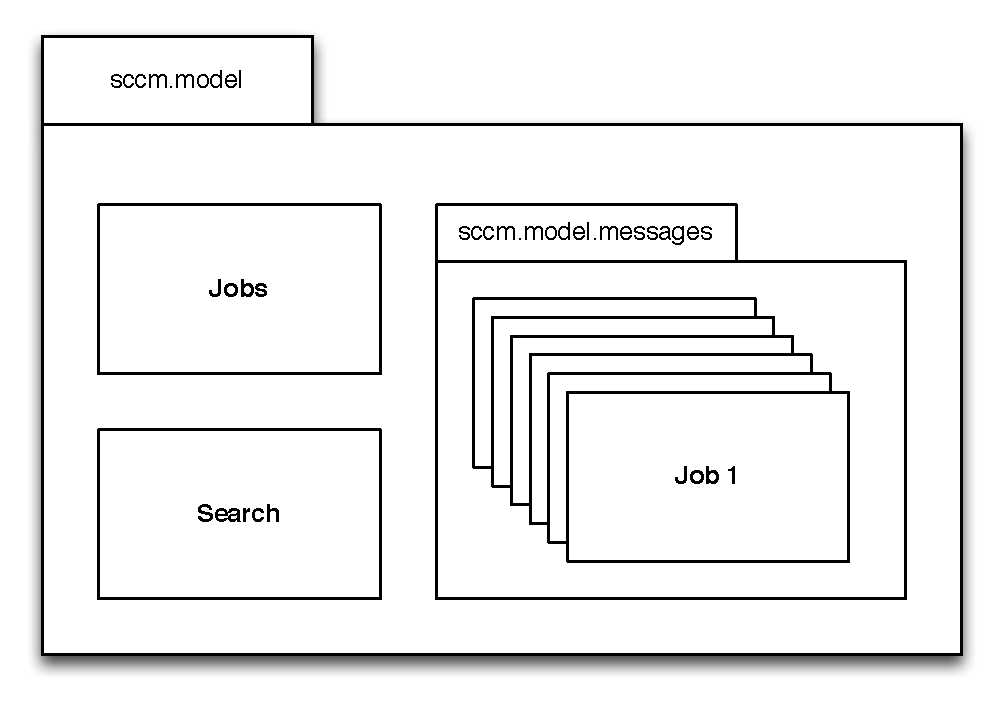
\includegraphics[width=12cm]{images/stores.pdf}
	\caption{Plug--in Models in the according namespaces}
	\label{fig:stores}
\end{figure}

\begin{listing}[H]
\begin{minted}[linenos=true,frame=none]{javascript}
sccm.model.messages = {
  getModel: function (name) {
    if(this[name] == undefined) {
      this[name] = new dojox.data.JsonRestStore({
        target: "http://9.152.130.251:8182/jobs/" + name
      });
    }
    return this[name];
  }
};
\end{minted}
\caption{Models for job results are created as Singletons}
\label{lst:models}
\end{listing}

An exemplary initialization of a results Model for the Job ``ibm-css'' is shown in Listing~\ref{lst:models2}. If the Model was not initialized before, it gets created then; otherwise, the reference to the existing Model is used.

\begin{listing}[H]
\begin{minted}[linenos=true,frame=none]{javascript}
theModel = sccm.model.messages.getModel('ibm-css');
\end{minted}
\caption{Initialization of a Model}
\label{lst:models2}
\end{listing}

\subsubsection*{Views and Controllers}
In the log-analysis plug--in, there is no View built completely from scratch. Although Dijits are \emph{visual} Dojo modules, they contain View code as well Controller code. These parts are hard to distinguish sometimes, as Dojo 1.6 does not provide a clearly structured MV* architecture.

As described in Section~\ref{sec:dojo}, the actual Views are Dijits such as \code{dijit.Tree} and \code{dojox.grid.DataGrid}. The log analysis plug--in does not extend or enhance them, it just \emph{uses} them.

The modules defined under the namespace \code{sccm.view} are not only Views, but View--Controller pairs. The Dijits, for example \code{sccm.view.StatsView}, are the Controllers, whereas the Views are defined inside their templates (or, programatically, inside the JavaScript code). In other words, the Controller \emph{wraps around} the View. This is the common way to define Dijits in \acl{icn}, as can be seen in the \emph{ICA Plug--in}, for example.

\begin{description}
	\item[\code{sccm.view.NavTree}] contains a \code{dijit.Tree} that displays all the plug--in's components. The search, jobs overview and job results can be accessed using this tree.
	The Controller code of this Dijit connects the Tree with the \code{sccm.model.Jobs} model
	\item[\code{sccm.view.StatsView}] is a Dijit containing an \code{idx.grid.PropertyGrid} (see Section~\ref{sec:customview} for more information on the PropertyGrid). It is used to the status of the log analysis system.
	\item[\code{sccm.view.JobsView}] contains a DataGrid to display the various log analysis jobs.
	\item[\code{sccm.view.ResultsView}] contains a DataGrid to display an overview of the job results.
	\item[\code{sccm.view.DetailsView}] contains a PropertyGrid to display details on a job result. This View is further described in Section~\ref{sec:customview}
\end{description}

\subsection{Implementation of a custom Model--View--Controller triad}
\label{sec:customview}
Part of the \ac{idx} distribution is a Dijit called \emph{PropertyGrid}. While the \emph{DataGrid} provided by stock Dojo is a good solution to get an overview on a large set of data, the \emph{PropertyGrid} is better suited to get a detailed view on a single object and its properties. In the log analysis plug--in, this was used in two places:
\begin{itemize}
	\item To display the properties of a \emph{Job} next to the list of results it returned,
	\item to display the system status and
	\item to display the details of the selected result item.
\end{itemize}
The last case is covered in this example. For every job, a \emph{tab} is created in a TabbedContainer Dijit (as described in Section~\ref{sec:plugindesign}) using the \code{sccm.layout.Messages} Dijit. The tab contains a DataGrid to display an overview of all the result items \code{sccm.view.ResultsView}, as well as a PropertyGrid to display details on the item that is \emph{selected} in the DataGrid \code{sccm.view.DetailsView}. Thus, the content of the PropertyGrid changes whenever a different item is selected in the DataGrid.
\begin{figure}[H]
	\centering
	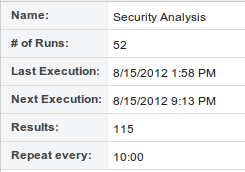
\includegraphics[width=6cm]{screens/propertygrid.png}
	\caption{The IDX PropertyGrid, displaying job details}
	\label{fig:propertygrid}
\end{figure}
Although the PropertyGrid is a data--driven Dijit, it is not designed to work together with a Dojo Store. The following example shows how this custom connection is established using the PropertyGrid as a View, a JsonRestStore through the DataGrid as a Model, and implementing Controller code to change the View's contents according to user actions.

One can argue that this is not a classic \ac{mvc} construction, as there is no Observer relationship between the View (\emph{PropertyGrid}) and the Model (the according \emph{JsonRestStore}). This is correct, but as the Model is read-only, the Observer is not necessary. It would be simple, though, to add it subsequently, if the PropertyGrid is used in a different scenario or the Model becomes writeable.

\subsubsection{Model}
The Model in this example is a simple \code{JsonRestStore}, as defined by Listing~\ref{lst:pgmodel}, but it is not used by the View directly. Instead, its data are accessed through the DataGrid, which is backed by the \code{JsonRestStore}. The listing defines a store for the ``ibm-css'' job. The \code{dataStructure} object is assumed to contain the structure for the DataGrid, which is not important here.
\begin{listing}[H]
\begin{minted}[linenos=true,frame=none]{javascript}
dataStore = new dojox.data.JsonRestStore({
  target: "http://localhost:8080/jobs/ibm-css"
});

dataGrid = new dojox.grid.DataGrid({
  store: dataStore,
  structure: dataStructure,
});
\end{minted}
\caption{Model and DataGrid for the PropertyGrid}
\label{lst:pgmodel}
\end{listing}

\subsubsection{View}
The PropertyGrid is created declaratively inside the template file of the tab.

\begin{listing}[H]
\begin{minted}[linenos=true,frame=none]{html}
<div
  dojoType="idx.grid.PropertyGrid"
  data="{}"
  properties=""
  dojoAttachPoint="detailsGrid"
></div>
\end{minted}
\caption{Declarative creation of the PropertyGrid}
\label{lst:pgview}
\end{listing}
Usually, the \code{data} attribute contains the data to be displayed, and the \code{properties} attribute contains information on how to format and label these data. In this case, both attributes are empty, as the information are set individually depending on the Model data.

\subsubsection{Controller}
As the Controller accesses two Dijits, it is placed one level higher, inside the \code{Messages.js} file of the \code{sccm.layout.Messages} Dijit. The code in Listing~\ref{lst:pgcontroller} is a simplified excerpt. It does not show the whole Dojo class developed for the tab of Job results, but only the parts relevant for the PropertyGrid. This code is also not in the context of the according Dojo class, but is extracted from it.

The code assumes a few objects to be present: \code{detailsGrid} is a reference to the PropertyGrid defined in Listing~\ref{lst:pgview}, \code{dataGrid} is a reference to the DataGrid, \code{job} contains the job description object (see Appendix and below).

The \code{structureForDetails()} function takes a \emph{result structure} object as the parameter. This object is part of the JSON description of a job; it describes the structure of a result item that is returned by an analysis job. In the Appendix, the JSON format of a job description is listed --- the \code{resultStructure} object, as part of it, is the object that gets passed in as a parameter here. \code{structureForDetails()} returns a string that lists all the properties that should be displayed in the PropertyGrid, and adds type information so that the properties are formatted properly. The returned string is in the format expected by the PropertyGrid for its \code{properties} attribute, as illustrated by Listing~\ref{lst:pgview}.

\code{detailsGrid} is a reference to the PropertyGrid Dijit. Using the \code{set()} method, the PropertyGrid's \code{properties} attribute is overwritten with a string created from the \emph{result structure} object, as described above.

The \code{dojo.connect()} function call in line~26 binds a callback, the \code{onRowClick()} function, to the \code{onRowClick} event of the DataGrid. This means, the callback is triggered when a row in the DataGrid is selected.

\code{onRowClick()} receives the selected result item from the DataGrid and sets it as the \code{data} attribute in the PropertyGrid. It then uses the \code{refreshPropertyGrid()} function to refresh the respective DOM nodes.

\begin{listing}[H]
\begin{minted}[linenos=true,frame=none]{javascript}
function structureForDetails(structure) {
  var a = "";
  for (var item in structure) {
    if(item != "__parent" && item != "__id") {
      var s = "";
      s = item;
      if(structure[item].type == "string")
        s += "(str)";
      else if(structure[item].type == "integer")
        s += "(int)";
      if(structure[item].type == "timestamp")
        s += "(dtm)";
      a += s + ",";
    }
  }
  // Remove trailing comma
  return a.substring(0,a.length - 1);
}

function onRowClick(event) {
  var item = dataGrid.getItem(event.rowIndex);
  detailsGrid.data = item;
  refreshPropertyGrid(this.detailsGrid);
}

function refreshPropertyGrid (pg) {
  for(var i = 0; i < pg._rows.length; i++)
    pg._rows[i].reformat();
}

// Set properties according to result structure
detailsGrid.set(
  "properties",
  structureForDetails(this.job.resultStructure)
);

dojo.connect(
  dataGrid,
  "onRowClick",
  dojo.hitch(this, onRowClick)
);
\end{minted}
\caption{Controller code for the PropertyGrid}
\label{lst:pgcontroller}
\end{listing}
